%************************************************
%\chapter{Use cases}
\chapter{Use-cases}
\label{cap:cases}
%************************************************

In the previous chapter we introduced a framework for web-based human and machine
computation, able to handle different types of application archetypes. In this
chapter we present the use-cases use to test this framework under different
scenarios. Since we wanted to test the framework with all the possible application
archetypes we implemented three use-cases: \emph{Automatic}, \emph{Human} and
\emph{Hybrid}:
\begin{description}
    \item[Automatic:] the automatic use-case is used to simulate a
    \emph{Distributed Computing} application. In this scenario we compute the
    SIFT algorithm on an image and return the obtained keypoints to the server.
    \item[Human:] the human use-case is used to test if we can perform \acl{HC}
    with our framework. To test this scenario we implemented a text disambiguation
    application.
    \item[Hybrid:] the hybrid use-case is used to test both the automatic and the
    human scenarios. Here we implemented a \ac{GWAP} on top of a face recognition
    algorithm.
\end{description}
\noindent We focused on the implementation of the \emph{Voluntary} scenario, see
\autoref{tab:matrix}, because the \emph{involuntary} case is almost straightforward
to obtain.
At the end of every use-case will be presented, if possible, a simple
benchmark/metric where the use-case results are compared with the ones obtained
with the available tools. 



\section{Automatic}
\label{sec:cases:automatic}
This use-case is the implementation of the scenario of \emph{voluntary-automatic}
presented in the matrix  in \autoref{tab:matrix}.

For the Automatic use case we choose to implement a widely used feature detection
algorithm, the \ac{SIFT}. To perform this load intensive algorithm we used the
power of the \ac{WebCL} framework to greatly speedup the computation.

% Come funziona
%% Creazione della libreria per comunicare con WebCl
%% Librearia per le operazioni sulle immagini usango WebCL
%% implementazione nella libreria dell'algoritmo
%% Fasi dell'algoritmo


\begin{figure}[htb]
    \centering
    
\includegraphics[width=\columnwidth]{Automatic1}
    \caption{The interface of the automatic use-case.}
    \label{fig:Automatic1}
\end{figure}


\begin{figure}[htb]
    \centering
    
\includegraphics[width=\columnwidth]{Automatic3}
    \caption{Step results of the algorithm.}
    \label{fig:Automatic1}
\end{figure}


\begin{figure}[htb]
    \centering
    
\includegraphics[width=\columnwidth]{Automatic3}
    \caption{Comparison with the reference data.}
    \label{fig:Automatic1}
\end{figure}


% 

%Our scenario is to detect features over 100.000 images using this algorithm


\subsubsection{Benchmark}
%non è possibile una vera comparazione data la velocità

\section{Human}
\label{sec:cases:human}
Dato un testo disambiguarlo usando YAGO (AIDA, https://d5gate.ag5.mpi-sb.mpg.de/webaida/), EntityPedia?, e altri
\citetitle{modernizr}


\section{Hybrid (automatic \& human)}
\label{sec:cases:hybrid}

With the previous sections we presented two applications able to handle the
human and the automatic scenarios. In this section we are presenting a use-case
where both the previous scenarios are blended together. This is used to test
if our framework is flexible enough to seamlessly support mixed application
archetypes. In the matrix at \autoref{tab:matrix} this use-case fits between the
human and the automatic computation.

\begin{figure}[htb]
    \centering
    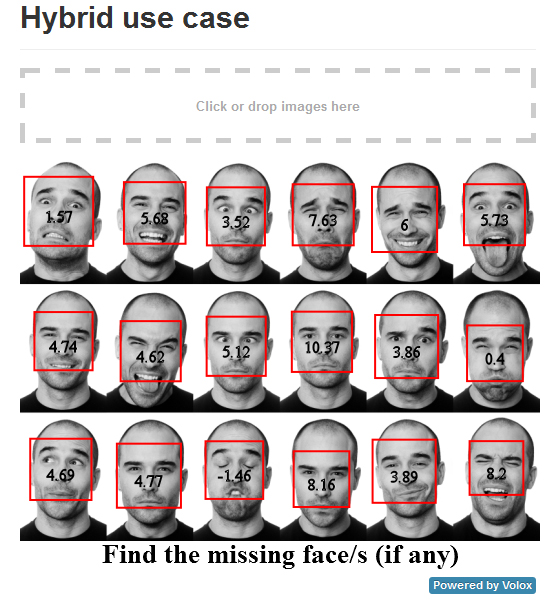
\includegraphics[width=0.75\columnwidth]{Hybrid}
    \caption{Interface of the hybrid use-case.}
    \label{fig:Hybrid1}
\end{figure}

This use-case has the purpose of \emph{detecting faces} in a picture, to accomplish
this Task are used an automatic face recognition algorithm plus a human interaction
that has the double purpose of validating the algorithm result and detect the
missing faces in the image.

This scenario is implemented in 2 steps, in the first step we run the algorithm
for detecting the faces (this is the \emph{automatic} scenario), the second step
is implemented as a \ac{GWAP}.\\

The game, under the name \textbf{ThemAmongUs} has been inspired by the 1988
film "\emph{They Live}" directed by John Carpenter. \emph{ThemAmongUs} is a
single player arcade shooter in which the player assumes a role of an agent that
fights against an alien race disguised as human beings. Equipped with a special
camera able to distinguish between human beings and non humans, the agent is
asked to shoot at the head of the beings that have not been identified by the
camera software. The camera may fail in some occasion, so the agent has to use
his judgment to fire only at the right targets.

\subsection{Introducing Score Degradation}
The new game mechanic that is presented to manage the task is called
Score-Degradation. This technique may be used in scenarios in which there are not
the possibility to compare the results provided by the players with techniques
such as the one provided in output-aggregation or inversion-problems games,
because the game that is being taken into consideration is a not a multiplayer
game but a single player one.

Goal of the technique is to force the user to always provide the right answer
with game mechanics that involve low reaction times , high penalties for mistakes
(such as early game termination) and incentives to achieve the best results
compared to all the other players.

Players are first evaluated based on well known trial examples tasks to understand
their reliability level. Failing the required task in these training examples
usually ends the gaming experience for the player, forcing him to start the game
from the beginning.

Once a sufficient level of trust for the player has been reached, the player is
then provided with a sequence of mixed tasks, some of them with an already well
established knowledge of the expected results, some of them with completely
unknown expected results. While the results of the first kind of tasks will
still be checked against the right results, for the second kind of tasks the
results provided by the players will always be considered good results.

The players will not be able to distinguish which of the instances of the tasks
are being checked against their provided results and which results are simply
considered "true as provided" without any further checks. This behavior is also
enforced by the fact that the player is not able to understand the moment in which
the "trial phase" will end and the fast reaction times force him to not even have
the time to think about providing misleading results, with the risk of having to
start the game from the beginning again.

In this way the player are always forced to try to give the best possible solution
for a specific task. The collected results can be further improved by using
traditional aggregation techniques such as majority voting or similar, depending
on the task that has to be solved.

\subsection{Gameplay}\label{case:hybrid:gameplay}
Goal of the game is to obtain the highest possible score given a limited amount
of time (1 minute). The player is provided with a series of images that present
bounding boxes of the face of human beings automatically identified by the special
camera of the agent. Each provided image will constitute a round of the game. If
in the image some face has not been surrounded by a bounding box, it means that
the portrayed subject is an alien and must be shot at by pressing the left click
button.

The player has a limited amount of time, typically 5 seconds, to shoot at all the
faces that have not been recognized, in order to obtain a certain amount of points.
During a round the player may also find improper bounding boxes, such as knees or
other part of the body that have been recognized as a face.

The player may right click on these boxes to remove them and obtain additional
points. When the player has shoot to all the unboxed faces, he may shoot at a
button on the right lower corner of the screen to play the next round of the game.
The game will end if the player will shoot at a recognized face by mistake.

At the end of each round (after the 5 seconds have passed or when the player has
pressed the end button), the system checks if the player has missed any face. If
it is the case and the image was a trial one or one for which the results were
known, the player will lose the game with a score equal to the number of points
he achieved so far. Otherwise the score for the current round are calculated in
the following way:
\begin{equation}
\begin{split}
    Score &= (RoundNumber*10)*(NumberOfAliensKilled)\\
          &+(100*(FalseBBRemoved))
\end{split}
\end{equation}

At the end of the global gaming time, a player who has not made any mistake will
receive 1000 additional points. The points are used to provide an incentive to
improve and beat other players by improving the score on further matches.